\documentclass[11pt, oneside]{article}   	% use "amsart" instead of "article" for AMSLaTeX format
\usepackage{geometry}                		% See geometry.pdf to learn the layout options. There are lots.
\geometry{letterpaper}                   		% ... or a4paper or a5paper or ... 
%\usepackage[parfill]{parskip}    		% Activate to begin paragraphs with an empty line rather than an indent
\usepackage{graphicx}				% Use pdf, png, jpg, or eps§ with pdflatex; use eps in DVI mode
\graphicspath{ {images/} }				% TeX will automatically convert eps --> pdf in pdflatex		
\usepackage{amssymb}
\usepackage{indentfirst}
\usepackage{amsmath}

%SetFonts

\newcommand\tab[1][1cm]{\hspace*{#1}}				% Define tab command and spacing
\renewcommand{\baselinestretch}{1.5}				% Define the line spacing
\newcommand{\rpm}{\raisebox{.2ex}{$\scriptstyle\pm$}}	% Define +/- for math script
\newcommand*\mean[1]{\overline{#1}}				% Define the bar over symbol to indicate mean

\title{NE155 Project Final Report}
\author{Milos Atz}
\date{May 10, 2016}							

\begin{document}

\maketitle

\section{Introduction}

Monte Carlo (MC) methods offer an alternative to deterministic methods of solving numerical problems. Rather than directly solving discretized equations, MC methods utilize repeated random sampling to obtain statistically likely solutions. Given enough repetitions, the MC result will converge to the true value. 

This project aims to design and implement an MC method to solve for the neutron flux in a two-region slab. Vacuum boundary conditions are assumed. Constant energy and material properties are assumed; scattering is assumed to be isotropic. The code will use a collision tally mesh to resolve the spatial flux shape. In addition, the relative error will be determined for each mesh space. Variance reduction methods are not implemented in this code.

\section{Mathematics}

Monte Carlo simulations rely on the probabilistic interpretation of physical phenomena by treating them as random variables. Every random variable has a probability density function and a cumulative distribution function. The probability density function (PDF) describes the probability $\in [0, 1]$ that some value of the random variable will be achieved. The PDF, $p(x)$, for a continuous random variable has the following characteristic.

\begin{equation}
p(a \leq x \leq b) = \int_{a}^{b}p(x)dx
\end{equation}

The probability of a variable attaining some value is always greater than 0. Integrating the PDF from $-\infty$ to $\infty$ accounts for all possible values and thus should return a value of 1. The integral of the PDF is the cumulative distribution function (CDF), $F(x)=P(X \leq x)$, which describes the probability that a continuous random variable $X$ will be less than or equal to the value $x$.

\begin{equation}
P(X \leq x) = F(x) = \int_{-\infty}^{x}p(x)dx
\end{equation}

The above equations are for continuous random variables; for discrete random variables, the integrals can be replaced with summations. Individual values for physical phenomena can be resolved by repeated random sampling according to the CDF. Based on a uniformly distributed random variable $\xi \in [0, 1]$, values for physical phenomena can be found using the associated CDF: $F(x) = \xi$. The challenge involves identifying the PDF/CDF for a given physical phenomena and finding $F^{-1}$ such that $x = F^{-1}(\xi)$.

There are many ways to sample random variables. Some simple methods include direct discrete sampling (i.e. to determine which reaction will take place), direct continuous sampling (determine the number of mean free paths), and rejection sampling (for non-invertible CDF). In this MC solver, as in all MC transport problems, each particle is followed from birth to its death. Through the particle's life, interactions and outcomes are randomly sampled from probability distributions using transport data. In this project, sampling is used to determine values and events. The sampling of these values is described in more detail in the next section. 

\begin{enumerate}
\item The direction of a particle when it is born or scatters.
\item The type of collision that might occur, either absorption or scattering.
\item The path length from the current particle location to it's next event.
\end{enumerate}

Each particle that is simulated creates a history of interactions throughout the problem space. For this problem, each interaction is a collision between a neutron and a nucleus in the medium. An estimator converts each history into a score, $x_{i}$. As more particles are followed, their scores accumulate into a tally, $\{x_{i}\}$. The expected value of this set is determined by the Strong Law of Large Numbers, which states that as the number of histories, N, tends toward infinity, $\mean{x}$ tends to E(x) \cite{MCNP}.

\begin{equation}
\mean{x} = E(x) = \frac{1}{N}\sum_{i=1}^{N}x_{i}
\end{equation}

The scores themselves are random variables, and so the tally has variance defined by the following. The variance is the square of the standard deviation.

\begin{equation}
S_{x}^{2} = \frac{1}{N-1}\sum_{i=1}^{N}(x_{i}-\mean{x})^{2}
\end{equation}

Tallies are used to model physical random variables of interest, for which the PDF is unknown and thus cannot directly sampled. In this problem, the physical variable of interest is the neutron flux, $\phi$, which is estimated by sampling score $x$. Each history, $i$, is a sample. As a sufficiently large number of histories are accumulated, the expected value of the tally will converge to the true value of the underlying PDF. In other words, the Monte Carlo attempts to relate $\mean{x}$ to the physical quantity of interest. 

\begin{equation}
\mean{\phi_L} = \frac{1}{L}\frac{1}{N}\sum_{i}x_{i} = \frac{\mean{x}}{L}
\end{equation}

Here, L is the length of the space over which the flux is being determined. Determining the precision of the Monte Carlo result relies on the Central Limit Theorem: for large values of N and independent and identically distributed (IID) random variables with finite expected values and variances, the distribution of those random variables approaches a normal distribution. This allows the definition of confidence intervals for $\mean{x}$ based on its estimated standard deviation. The estimated variance of $\mean{x}$ is shown below \cite{MCNP}.

\begin{equation}
S_{\mean{x}}^{2} = \frac{S_{x}^{2}}{N}
\end{equation}

Thus, as the number of histories (N) is increased, the estimated standard deviation decreases. Another measure of result precision is relative error. The relative error is the estimated standard deviation of the mean relative to the mean, and is given by the following.

\begin{equation}
R = \frac{S_{\mean{x}}}{\mean{x}}
\end{equation}

It should be noted that no statistical indicator of a Monte Carlo result can tell about the accuracy of the solution; statistics only indicate precision. Accuracy is influenced by the correctness of the physical and mathematical used in the problem, errors in the code, or errors in the problem specification. For most Monte Carlo simulations, the accuracy is unknown and can only be validated by comparison with experiment.

\section{Algorithms}

The algorithm for this code can be described by the flowsheet in Figure \ref{fig:flowsheet}. To sample for direction, generate a random number $\xi$ on the uniform distribution $[0,1)$. The direction is positive (right) if $\xi \geq 0.5$. The direction is negative (left) if $\xi < 0.5$. When direction is sampled, the cosine of the angle is also sampled. Scattering is assumed to be isotropic, so any angle $\in [0, 2\pi]$ is possible. Because the value of interest is the cosine of the angle, $[\pi, 2\pi]$ return the same values as $[0, \pi]$. In addition, because sampling for direction already eliminates half of the potential angles from consideration, the cosine of the angle is simply identified by generating a random number $\xi$ on the uniform distribution $[0, 1)$. This, multiplied by the direction and the path length, gives the new location (and potentially the collision site) of the particle.

\begin{figure}
  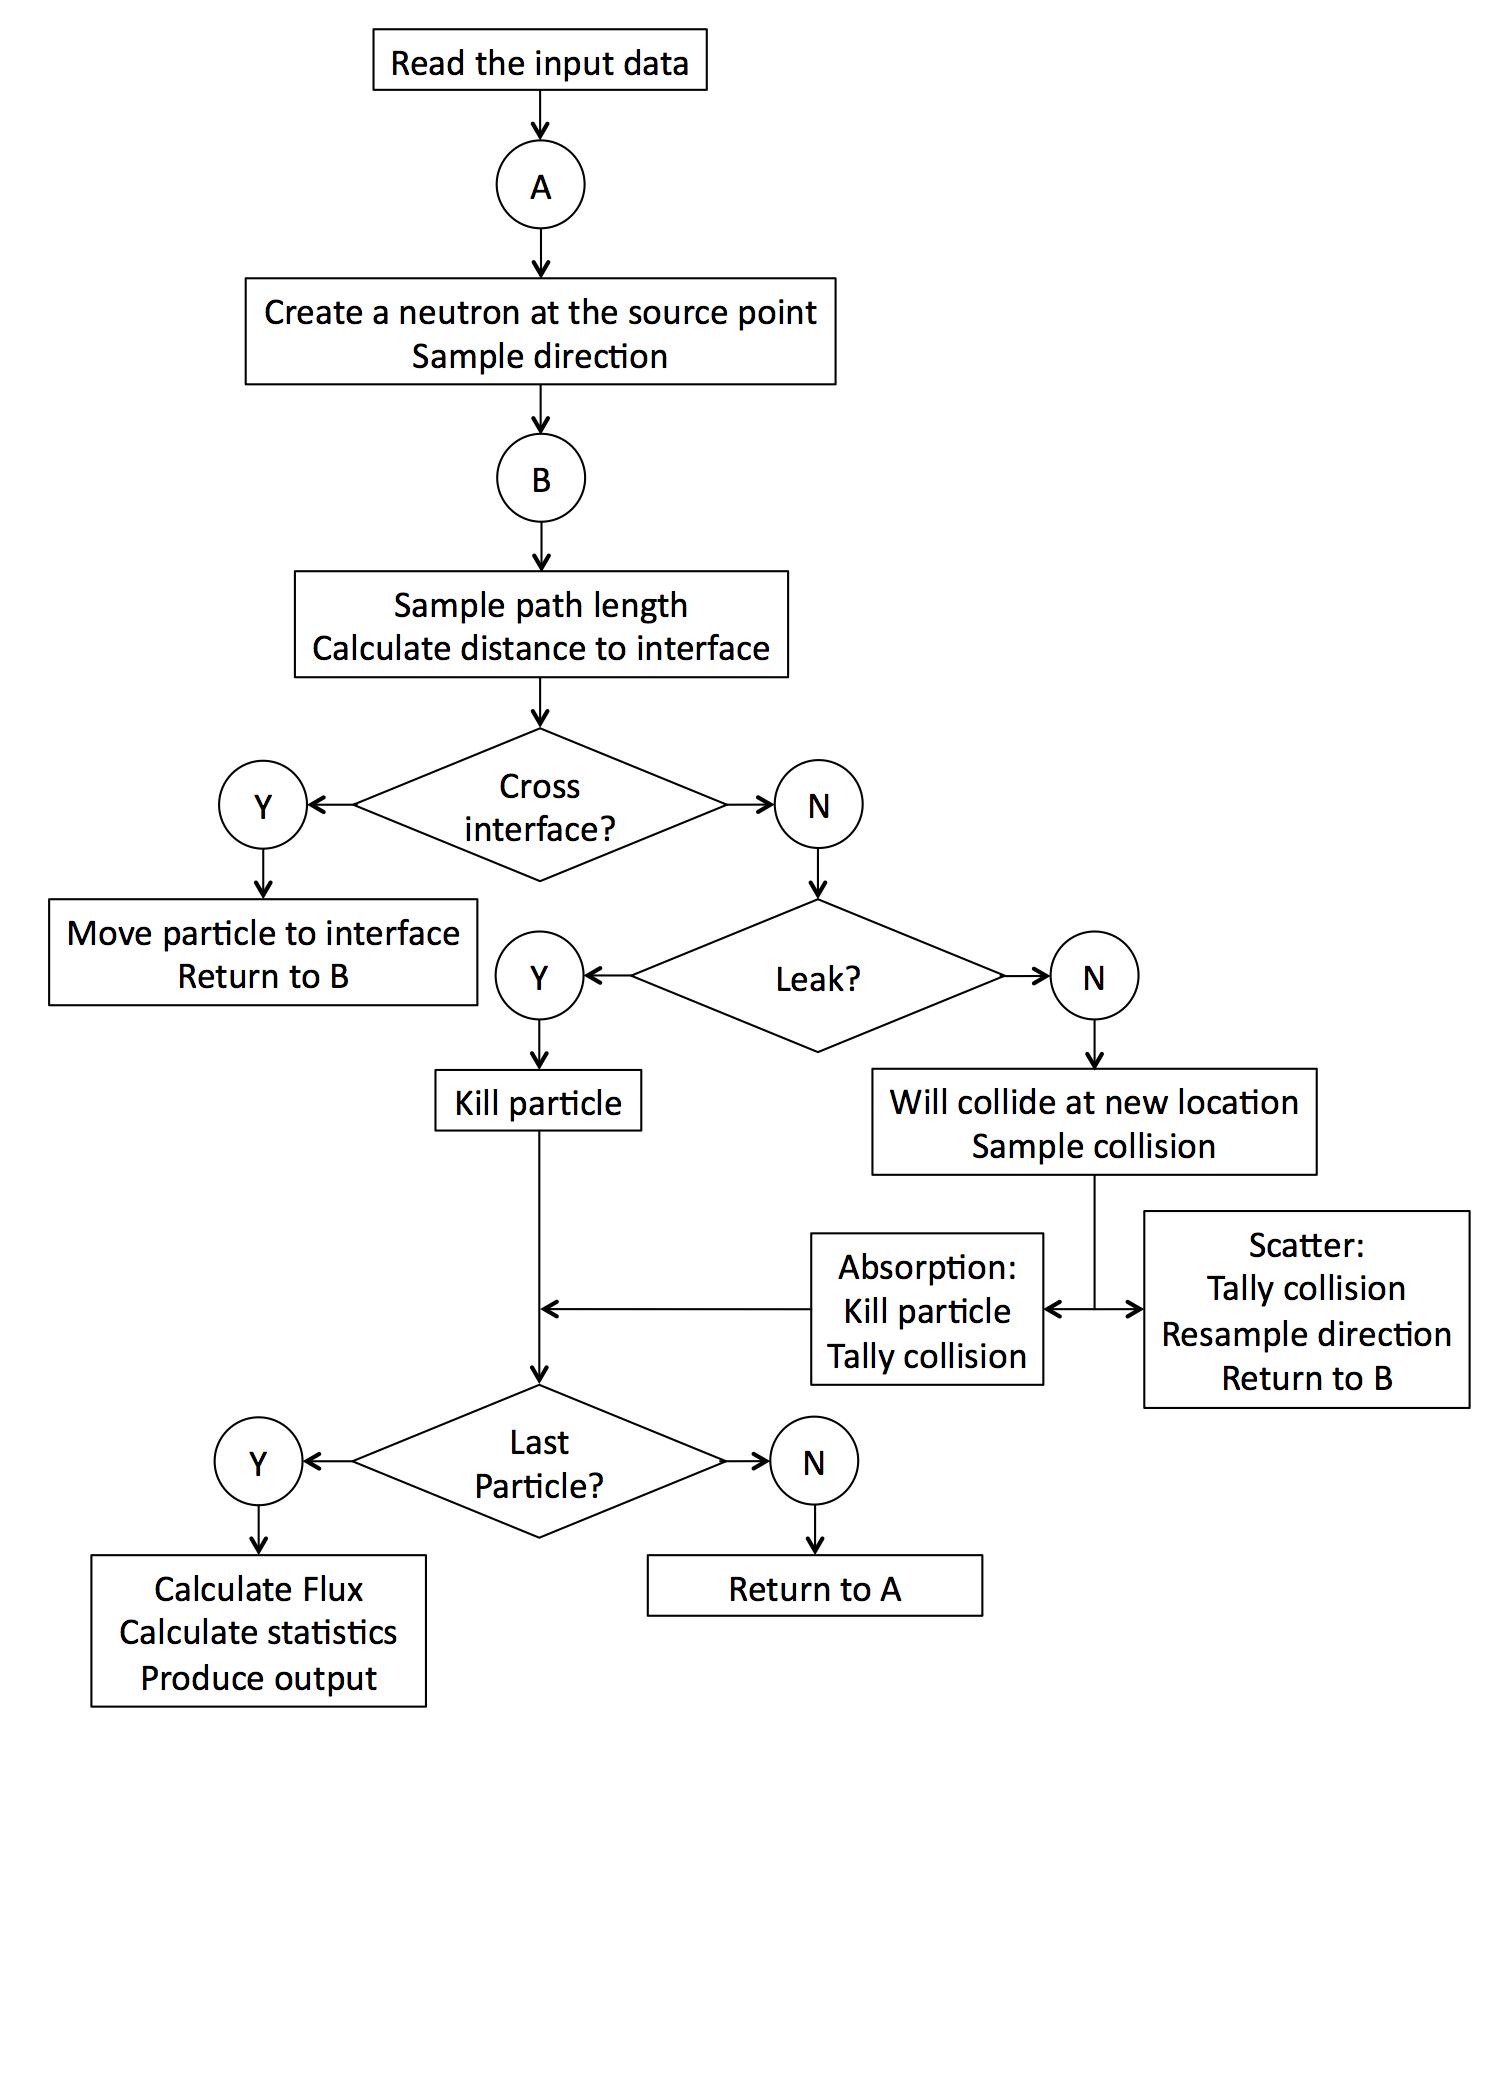
\includegraphics[width=\linewidth]{flowsheet}
  \caption{Flowsheet describing the algorithm for the Monte Carlo routine carried out in this code.}
  \label{fig:flowsheet}
\end{figure}

The path length is sampled for the region the neutron is currently in (or, if it is crossing the interface between the two regions, for the region the neutron is entering).
 
\begin{equation}
F_s(s)=\Sigma_t e^{-\Sigma_ts}
\end{equation}

\begin{equation}
s = -\ln(\xi)/\Sigma_t
\end{equation}

If the particle is moving toward the interface, the distance between the particle and the interface is measured to determine whether the particle changes region. If the distance between the particle and the interface is less than the sampled path length, the particle will enter the other region. The particle is moved to the boundary and the path length is resampled for the region the particle is entering; the direction and angle remain the same.

If the particle is moving toward a boundary, the sampled path length is compared to the distance between the particle location and the boundary. If the sampled path length is greater than the distance to the boundary, the particle leaks and is terminated. 

If the particle does not change regions and does not leak, it will collide within the region it is in. The particle is moved to its new location and the type of collision is sampled. Two types of collision are possible, scattering and absorption; these are characterized by their cross sections, $\Sigma_{s}$ and $\Sigma_{a}$, respectively. The total cross section is defined as $\Sigma_{t}=\Sigma_{s} + \Sigma_{a}$. Thus, the probability of a reaction $i$ is given by the following.

\begin{equation}
p_{i} = \frac{\Sigma_{i}}{\Sigma_{t}}
\end{equation}

Each reaction type has a discrete probability, which can be sampled directly by generating a random number $\xi$ on the uniform distribution $[0,1)$ and determining $k$ such that $F_{k-1} \leq \xi \leq F_{k}$. The reaction $i_{k}$ is the one that occurs. If the particle is absorbed, it is terminated. If the particle scatters, direction and angle are resampled and the process is repeated.

For every history, a tally vector is generated to track the scores. The entries in the vector correspond to the spatial bins specified in the input (the user inputs problem bounds and the width of the spatial bins). Every time a collision occurs, a score is added to the tally corresponding to the spatial bin in which the collision took place. Each score has the same weight. After each history, the scores in each bin are added to a cumulative tally. Once all the histories have been completed, this cumulative tally is used to calculate the $\mean{\phi}$. In addition, it is used to determine the sample variance. For this, the sum of the squared scores is also required. Thus, for each history, the square of each score in the tally is added to a cumulative total. After all histories are completed, this is equal to the sum of the squared scores and can be used to calculate the sample variance.

The flux result given needs to be scaled by source strength, which is input by the user. Once all histories are complete, the flux and statistics are evaluated for each spatial bin.

\section{Code Use}

The code is executed by running the python script "run" from the Terminal. All of the necessary python subscripts are included in the same directory and are imported and called in when needed. The user controls many aspects of the problem by adjusting the input values at the top of "run.py". The user specifies coordinates of the left and right bound of the slab, the location of the interface, the strength of the source, and the width of the tally mesh bins. In addition, the user can modify the scattering and absorption cross sections in each region.

One important parameter controlled by the user is the number of particles (i.e. histories) to be run in the problem. The appropriate number of particles depends on the required statistical precision, which in turn depends on the width of the tally mesh bins. Running more histories will always yield a more precise result but requires increasingly more time.

Running the code results in the generation of a scatter plot showing the flux at the center of each tally mesh bin. Error bars are included on the points, showing the relative error of the estimated mean. If the error is sufficiently small, the error bars will not clear the points but are still overlaid on the points. The maximum relative error for the problem is printed in the Terminal, giving the user a bound for the precision of the result.

\section{Testing and Numerical Results}

As previously mentioned, it can be very difficult to check the accuracy of results from Monte Carlo methods. However, for this simple problem, the problem can solved using diffusion theory. Comparing the diffusion result for flux against the Monte Carlo result can yield insight into the quality of the simulation. Equation \ref{DE} shows the one-speed diffusion equation in one dimension (x) \cite{duderstadt}.

\begin{equation}
\label{DE}
\frac{1}{v}\frac{\partial \phi}{\partial t} - \nabla D(x) \nabla \phi (x,t)+\Sigma_a (x) \phi (x,t) = S(x,t)
\end{equation}

To solve this equation, it is assumed that material properties are homogeneous and that the flux does not change with time (steady state). The source is considered as a plane source that occurs at some value $x_{s}$. The solution is obtained by solving around the location of the source, which splits the slab into two regions. The flux in each region is solved separately. The boundary condition at the plane source is defined in terms of the current given by Equation \ref{sourceBC}.

\begin{equation}
\label{sourceBC}
\lim_{x \to x_{s}}J(x) = \frac{S}{2}
\end{equation}

This represents a special case of the general interface boundary condition based on assuming symmetry in material properties and geometry across the interface. The boundary condition says that the current on either side of the origin must be half of the source strength. Vacuum boundary conditions are utilized at the boundaries on either side of the slab. The vacuum boundary condition is given by Equation \ref{vacuumBC}.

\begin{equation}
\label{vacuumBC}
\phi (a_{ext})=0
\end{equation}

Here, $a_{ext}$ represents the extrapolated distance for whichever side of the slab, right or left, on which the boundary is being considered. Applying these boundary conditions, the flux in the slab defined by left and right boundaries $a$ and $b$, respectively, with $x_{s} = 0$ is found to be defined by Equations \ref{soln_pos_fixedsrc} and \ref{soln_neg_fixedsrc}.

\begin{equation}
\label{soln_pos_fixedsrc}
\phi(x) = \frac{SL}{2D}\bigg(1+e^{-2\frac{b_{ext}}{L}} \bigg)	^{-1} 	\bigg(e^{\frac{-x}{L}}-e^{-2\frac{b_{ext}}{L}}e^{\frac{x}{L}} \bigg) \tab 0 < x \leq b_{ext}
\end{equation}


\begin{equation}
\label{soln_neg_fixedsrc}
\phi(x) = \frac{SL}{2D}\bigg(1+e^{-2\frac{a_{ext}}{L}} \bigg)	^{-1} 	\bigg(e^{\frac{-x}{L}}-e^{-2\frac{a_{ext}}{L}}e^{\frac{x}{L}} \bigg) \tab a_{ext} \leq x < 0
\end{equation}

Additionally, if it is assumed that back scattering across the plane source is negligible, the location of the plane source can be used to define the interface between two regions. The Monte Carlo solution considers a two region slab with variable placement of source; this diffusion solution makes nearly perfect agreement between the problems. The only difference is that for the diffusion solution, the interface between the regions is fixed at the location of the plane source. In the Monte Carlo solution, the locations of the interface and source are independent. Equations \ref{soln_pos_fixedsrc} and \ref{soln_neg_fixedsrc} can be modified to allow for variable placement of the location of the source and interface, as demonstrated by Equations \ref{soln_pos} and \ref{soln_neg}, respectively.

\begin{equation}
\label{soln_pos}
\phi(x) = \frac{SL}{2D}\bigg(1+e^{-2\frac{(b_{ext}-x_{s})}{L}} \bigg)^{-1} \bigg(e^{-\frac{(x-x_{s})}{L}}-e^{-2\frac{(b_{ext}-x_{s})}{L}}e^{\frac{(x-x_{s})}{L}} \bigg) \tab 0 < x \leq b_{ext}
\end{equation}


\begin{equation}
\label{soln_neg}
\phi(x) = \frac{SL}{2D}\bigg(1+e^{-2\frac{(a_{ext}-x_{s})}{L}} \bigg)^{-1} \bigg(e^{-\frac{(x-x_{s})}{L}}-e^{-2\frac{(a_{ext}-x_{s})}{L}}e^{\frac{(x-x_{s})}{L}} \bigg) \tab 0 < x \leq b_{ext}
\end{equation}

When specifying the input, the user chooses whether the analytical solution should be included. If it is included, the interface is forced to be at the location of the source. Together, the Monte Carlo and analytical solutions give results like those demonstrated in Figures \ref{fig:an_result1} and \ref{fig:an_result2}.

\begin{figure}
\centering
  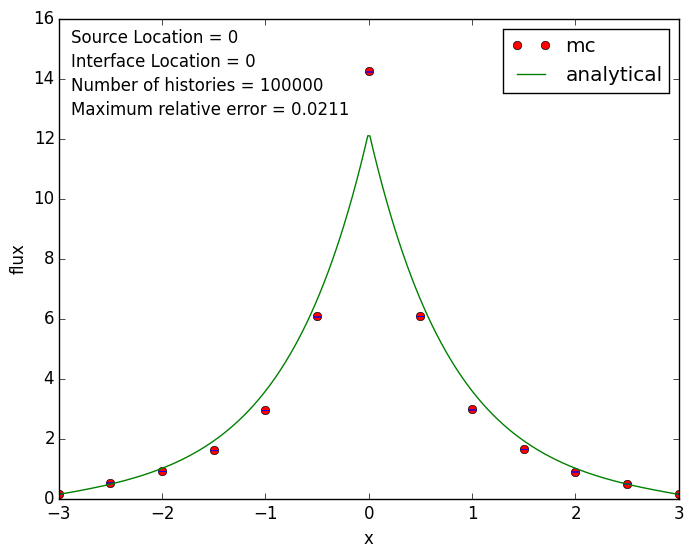
\includegraphics[width=12cm, keepaspectratio,]{an_result1}
  \caption{Example of code output comparing the Monte Carlo and analytical diffusion solutions for flux in the system. Here, $x_s = 0$ and the material properties are the same on either side of the source plane.}
  \label{fig:an_result1}
\end{figure}

\begin{figure}
\centering
  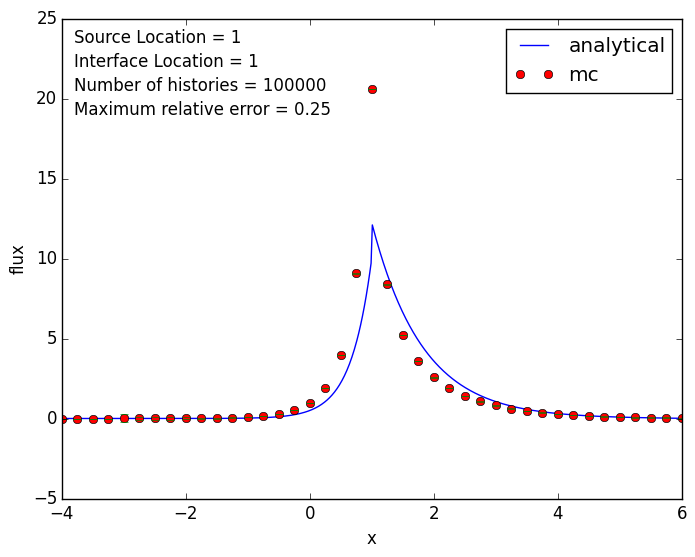
\includegraphics[width=12cm, keepaspectratio,]{an_result2}
  \caption{Example of code output comparing the Monte Carlo and analytical diffusion solutions for flux in the system. Here, $x_s = 1$ and the cross-sections are different on either side of the source plane.}
  \label{fig:an_result2}
\end{figure}

The different cross-sections on either side of the source plan in \ref{fig:an_result2} lead to the discontinuity in the analytical solution at that point. Though not rigorously correct, it gives an approximation of the solution and serves to validate the Monte Carlo result. If the analytical result is not included, the interface can be located anywhere, generating flux profiles like that in Figure \ref{fig:mc_result1}.

\begin{figure}
\centering
  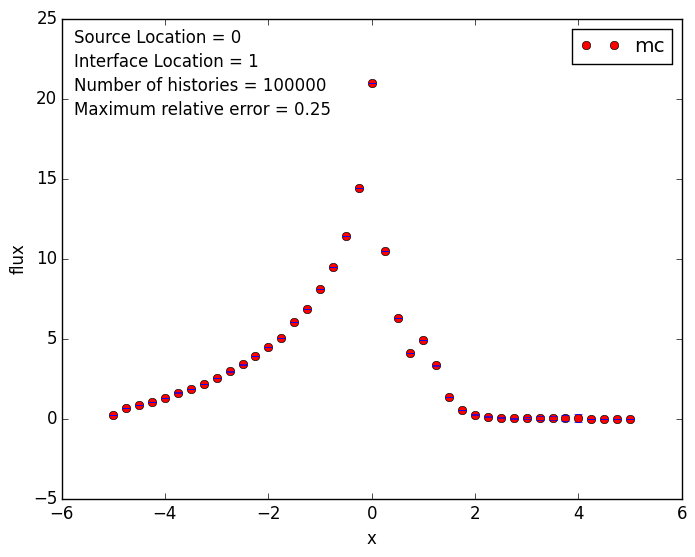
\includegraphics[width=12cm, keepaspectratio,]{mc_result1}
   \caption{Example of code output showing Monte Carlo output with the different locations for the source ($x = 0$) and the interface ($x=-2$).}
  \label{fig:mc_result1}
\end{figure}

In Figure \ref{fig:mc_result1}, the total and scattering cross-sections on the right of the interface are two and three times as large, respectively, as those on the right. This means that the probability of absorption to the left of the interface ($x = -1$) is half of that on the right. The result is a slight peak in flux, stemming from the fact that particles are more likely to be absorbed to the right of the interface than to the left.

The statistical quality of the result can be altered by careful problem setup. Increasing the number of histories decreases the relative error and standard deviation. The relative error can also be decreased by making the spatial bins more coarse. If there are less spatial bins, more particles will fall into each, improving the statistics in each bin. The standard deviation is largest where the flux is highest; conversely, because the relative error is equal to the standard deviation divided by the mean flux, the relative error is largest near the boundaries where the flux is near zero. This indicates the significance of the relative error. Because more particles exist in the high flux regions, the result should be best resolved where the flux is highest, leading to the lowest relative error.

For this simple problem, it does not take many particles to arrive at a solution with acceptable statistics; the analog Monte Carlo is satisfactory. This works well when most of the particles contribute to the tallies. When this is not the case, the statistical uncertainty of the answer can be enormous. To avoid this, non-analog Monte Carlo is used, which attempts to follow interesting particles more than non-interesting ones, therefore increasing the chances that more particles will contribute to the tally. To avoid artificial inflation of the tally results, the contribution of each particle to the tally is modified to remove the effect of this biasing. There are many ways to do this, referred to generally as variance reduction \cite{MCNP}. Though none of these methods are not included in this code, many can be readily implemented in future versions.

% REFERENCES
\begin{thebibliography}{9}

\bibitem{MCNP}
\textit{MCNP5 - A General Monte Carlo N-Particle Transport Code, Version 5}.
Volume 1: Overview and Theory. X-5 Monte Carlo Team, Los Alamos National Laboratory (rev. 2008).

\bibitem{duderstadt}
J. J. Duderstadt, L. J. Hamilton
\textit{Nuclear Reactor Analysis}.
John Wiley \& Sons, Inc. 1976.

%\bibitem{NE155_notes_1}
%R. Slaybaugh
%\textit{UCBNE155 Class Notes Spring 2016}.
%April 6, 2016

%\bibitem{NE155_notes_2}
%R. Slaybaugh
%\textit{UCBNE155 Class Notes Spring 2016}.
%April 8, 2016

%\bibitem{NE250_notes_1}
%R. Slaybaugh.
%\textit{UCBNE250 Class Notes Fall 2015}.
%October 21, 2015.

%\bibitem{NE250_notes_2}
%R. Slaybaugh.
%\textit{UCBNE250 Class Notes Fall 2015}.
%October 26, 2015.

\end{thebibliography}

%%% NOTES AND UNUSED TEXT %%%
%When MC algorithms involve following each particle, they are said to be analog methods because they are analagous to natural transport. This works well when most of the particles contribute to the tallies. When this is not the case, the statistical uncertainty of the answer can be enormous. To avoid this, nonanalog Monte Carlo is used, which attempts to follow interesting particles more than noninteresting ones, therefore increasing the chances that more particles will contribute to the tally. To avoid artificial inflation of the tally results, the contribution of each particle to the tally is modified to remove the effect of this biasing. There are many ways to do this, referred to generally as variance reduction \cite{MCNP}.

%This code aims to solve a simplified version of the neutron transport equation (NTE). In this section, the NTE will be introduced and simplifying assumptions will be applied in order to arrive at the equation solved by this code. 
%\begin{multline}

%\frac{1}{v}\frac{\partial \psi}{\partial t}(\rvec,E,\omvec,t) + \omvec\cdot  \nabla \psi(\rvec,E,\omvec,t) + \Sigma_t(\rvec,E)\psi(\rvec,E,\omvec,t) = \\
%\int_0^{\infty}\int_{4\pi}\Sigma_s(\rvec, E'\rightarrow E,\omvec'\rightarrow\omvec) \psi(\rvec,E',\omvec',t)d\omvec'dE'+S(\rvec, E, \omvec,t)
%\end{multline}

%Equation one is the neutron transport equation, which describes the flux of neutrons with at a position $\rvec$ with energy $E$ traveling in direction $\omvec$ at time $t$. These conditions comprise the seven dimensional phase space of the NTE. The first term represents the time dependence of the flux, $\psi$. The second term is the streaming term, representing the passage of particles through the boundaries of the differential volume. The third term is the collision term, representing all reactions that remove neutrons from the flux. The fourth term is the scattering term, counting neutrons that scatter into the relevant energy and direction from all other possible energies or directions, thus adding to the flux. The last term is an external source of neutrons, which can be replaced by fission if applicable.

%\begin{itemize}
%\item If $w_i >w_{max}$, splitting is required
%\item If $w_i < w_{min}$, rouletting is required
%\end{itemize}

%\item Implicit capture (survival biasing) states that the tally should be $w_i(\Sigma_a/\Sigma_t)$ and the neutron's weight is  reduced by $w_{i+1}=w_i(1-\Sigma_a/\Sigma_{tot})$, where $\Sigma_a = \Sigma_{tot}-\Sigma_s$. 
%\item If $w_{i+1} \leq w_{min}$, rouletting is performed to see if the particle survives. The rouletting procedure is described in a later section. If the particle survives, return to step 2 with the new weight. If not, it is killed and it's weight is set to 0.
%\end{itemize}

\end{document}
